\documentclass[a4]{scrartcl}

\usepackage[ngerman]{babel}
\usepackage[utf8]{inputenc}
\usepackage{mathtools}
\usepackage{amsmath}
\usepackage{amssymb}
\usepackage{geometry}
\usepackage{scrpage2}
\pagestyle{scrheadings}
\clearscrheadfoot


\geometry{
  paper=a4paper, % Change to letterpaper for US letter
  top=2cm, % Top margin
  bottom=1.5cm, % Bottom margin
  left=2cm, % Left margin
  right=3cm, % Right margin
  %showframe, % Uncomment to show how the type block is set on the page
}

\setlength{\parindent}{0em}

\ohead{\\
Pina Kolling}

\begin{document}

\section*{Vorlesung 5}

\textbf{Sichten auf Transformationsstratiegien}
\begin{itemize}
\item \textbf{Innovationsperspektive:}

\begin{itemize}
\item \textbf{Phase 1 Experimentieren am Rande der Organisation}

\begin{itemize}
\item ergänzende Experimente: \\
Das bestehende Geschäftsmodell bleibt bestehen, Innovation beruht auf das vorhandene Geschäftsmodell.
\item disruptive Experimente: \\
Das Geschäftsmodell wird grundlegend innoviert. \\

\hspace*{0.8em} 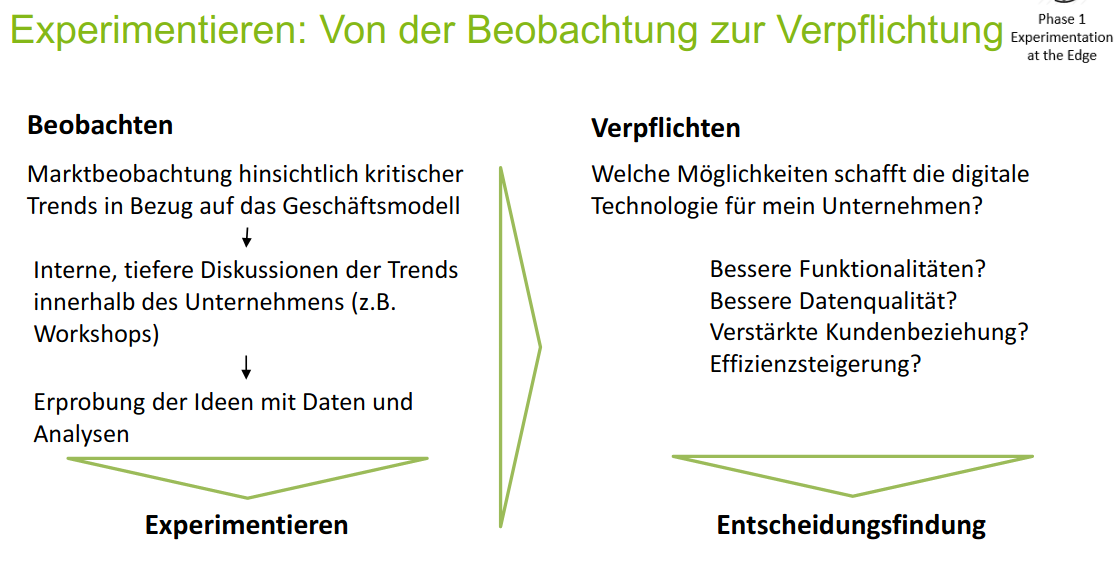
\includegraphics[scale=0.25]{experiment.png} \\


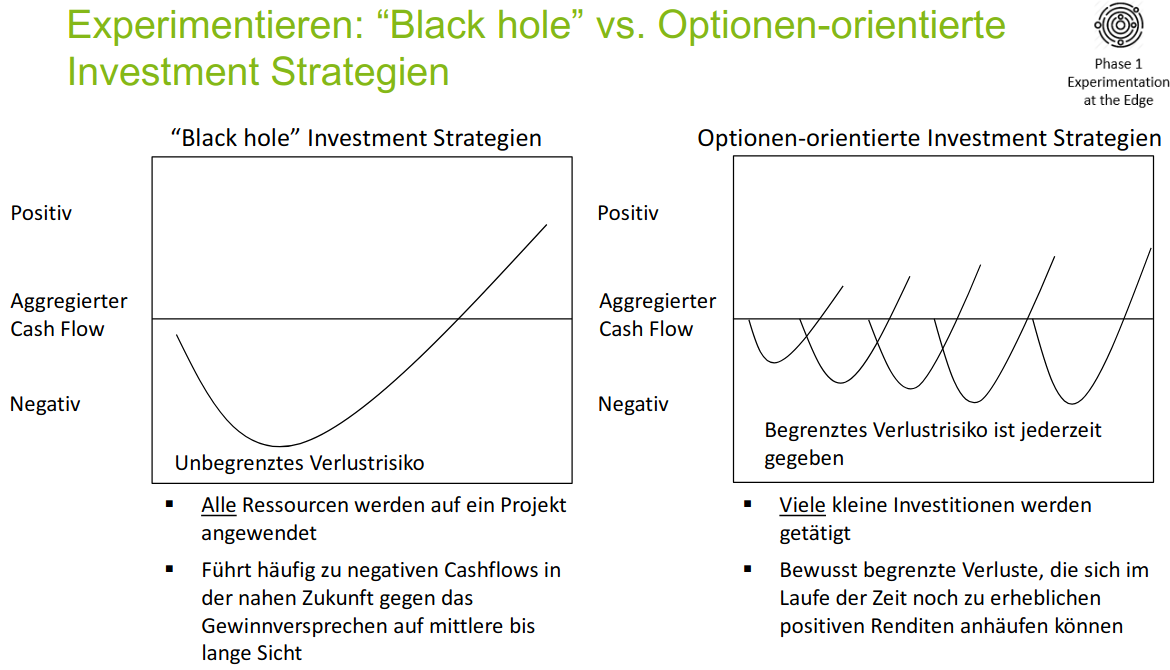
\includegraphics[scale=0.22]{bh.png}

\end{itemize}

\item \textbf{Phase 2 Kollision im Kern}

\begin{itemize}
\item Kollision in der Strategie

\begin{itemize}
\item z.B: Kollision mit Strategien von anderen etablierten Unternehmen der Branche
\end{itemize}

\item Kollision der Organisation \\
Effizienz-Nachteile in:

\begin{itemize}
\item Durchlaufzeiten
\item Entscheidungsgeschwindigkeit
\item Führungsmodelle
\end{itemize}



\end{itemize}





\item \textbf{Phase 3 Neuerfindung an der Wurzel}

\begin{itemize}
\item Veränderung der Kernelemente des Geschäftsmodells durch digitale Technologien
\end{itemize}

\end{itemize}

\item \textbf{Architekturperspektive}

\begin{itemize}
\item Geschwindigkeit  $\rightarrow$ hoher Innovationsgrad
\item Stabilität $\rightarrow$ zuverlässige Kernprozesse
\end{itemize}



\item Führungsperspesktive
\end{itemize}








\end{document}